\documentclass[12pt]{article}

\title{Data Analysis Project Report}
\author{James Hughes}

\usepackage[nottoc,numbib]{tocbibind}
\usepackage{graphicx}

\newcommand\NA{\mathit{NA}}

\begin{document}

\begin{titlepage}
    \begin{center}
        \vspace*{1cm}

        \Huge
        \textbf{Deep Learning for Structured Illumination Microscopy Image Processing}

        \vspace{0.5cm}
        \LARGE

        James Hughes

        Supervised by Dr Edward Ward

        \vspace{2cm}
        \Huge
        \textbf{Project Report}

        \vfill

        MPhil, Data Intensive Science

        \vspace{0.8cm}

        \Large
        Department of Physics \& Department of Chemical Engineering and Biotechnology

        University of Cambridge

        United Kingdom

        28th June 2024

    \end{center}
\end{titlepage}

\pagenumbering{roman}

\newpage
\section*{Acknowledgements}
\addcontentsline{toc}{section}{\protect\numberline{}Acknowledgements}

Firstly I would like to thank my supervisor, Dr Edward Ward, for all of his support over the course of this project.
The project involved a lot of concepts from microscopy and image processing that were very new to me,
but Dr Ward made it clear from early on in the project that this would not be a problem,
and was quick to provide reading materials to help me get to grips with the subject.
Having been trained in Mathematics during my time as an undergraduate,
the chance to go into the laboratory and capture real microscope images that were later used in the work was incredibly exciting.
Dr Ward was eager to provide this opportunity and welcomed me to the Chemical Engineering and Biotechnology (CEB) Department and his research group.

I also had the opportunity to attend some of the Laser Analytics Group (LAG) lab meetings,
where I had the privilege of learning about some of the world-leading research being undertaken by the group.
Later, I shared details about my own project in two presentations to the group.
I would like to thank all of the members of the LAG for welcoming me, listening to my presentations and providing great feedback.
In particular I wish to thank Professor Clemens Kaminski for his helpful suggestions and words of encouragement.

I would also like to thank Jeremy Wilkinson, Esther Gray, and Emilio Luz-Ricca.
I had very insightful conversations about the project with all of them that helped me see the work in a new light.

Lastly, I would like to thank my parents for being a continual source of support and strength throughout my education,
in particular for encouraging me to make the most of every opportunity that comes my way.

\newpage
\begin{abstract}
    \addcontentsline{toc}{section}{\protect\numberline{}Abstract}

    Structured illumination microscopy improves the resolution of imagery beyond Abbe's diffraction limit imposed on widefield images.
    However, imaging live-cell dynamics is restricted by phototoxicity effects, limiting the maximum duration of such imaging.
    In 2023, Li et al. developed a `two-step denoising' approach, which involves greatly reducing the illumination intensity of the microscope,
    and in turn using deep learning to recover the lost signal in the image.
    This project aims to investigate the reproducibility of their work.
    Primarily the work presents an open-source data processing pipeline which implements their method,
    allowing further investigation on different datasets, or extensions to the work.
    This work presents the results of applying the method to 2D SIM data consisting of microtubule images.
    Later, the applicability to 3D SIM was explored by using data Visible Human Project to simulate imagery acquired from a 3D SIM microscope.
    The work

\end{abstract}

\newpage
\tableofcontents

\newpage
\pagenumbering{arabic}
\section{Introduction}

Fluorescence microscopy is an essential tool for microbiologists,
enabling them to view complex biological phenomena unfolding at the sub-cellular level.
Fluorescent dyes are employed to attach to specific organic compounds,
which then release photons in response to illumination from a laser at a suitable wavelength,
producing images that highlight specific structures of interest to researchers.
As a type of optical microscopy, the resolution of these systems is limited by the effects of diffraction.
This limit was quantified by Abbe \cite{abbe} in 1873 as a minimal resolvable distance between two points,

\[d=\frac{\lambda}{2\NA}\]

where $\lambda$ refers to the emittance wavelength, and $\NA$ refers to the numerical aperture,
a property of the optical system and the imaging medium.
This resolution limit is summarised by the optical transfer function $O(\vec{k})$ of the microscope,
which describes the set of spatial frequencies of the sample structure that can be captured by the optical system,
and to what extent they are attenuated in the resulting image (in frequency space).
Axial resolution of optical microscopes is typically much worse than their lateral resolution.
This fact is evidenced by the optical transfer function's omission of most k-vectors that lie along and near to the z-axis.
This is further compounded in practice with issues such as spherical abberation.
This represents a serious obstacle to researchers attempting to view cell dynamics in greater detail.

Structured Illumination Microscopy (SIM) is a technique that combines a specialised microscope set-up,
alongside computational processing of the acquired images,
in order to surpass the classical Abbe diffraction limit.
The theoretical foundations of the technique were first established in 2008 \cite{originalSIM},
but since then there have been a range of improvements made to the technique.
While SIM does not necessarily provide the greatest improvements in resolution compared to other methods such as confocal,
it has other advantages for researchers interested specifically in capturing imagery of dynamic biological processes over extended periods.
This relates primarily to the issue of phototoxicity effects.
Every time a fluorescence microscopy image of a cell sample is taken, the cell itself is bleached and damaged in the process.
This is particularly troublesome when one wishes to view dynamic processes in live cells,
because the very process of imaging has an effect on the process being captured,
thereby limiting the duration of imagery that can be obtained that is faithful to the true process.
SIM offers a trade-off between resolution improvements and low photo-toxicity effects.

The paper by Li. et al. \cite{keypaper} attempts to augment the SIM image processing pipeline with deep-learning techniques to improve this trade-off.
Their research explores multiple ways in which hardware and computation can be used to improve the resolution of SIM imaging.
This project investigates their `two-step denoising method'.
The core of this technique involves dramatically lowering the illumination dose of the SIM laser,
in order to mitigate phototoxicity effects.
In turn, they train two networks to denoise the acquired and reconstructed images,
to attempt to compensate for the low intensity illumination and reclaim lost image resolution.

This project aims to present a full pipeline that implements their method.
The tools developed in the repository aim to make the method accessible to other research groups looking to apply it to their own data,
with minimal work required for set-up, and compatibility with common tools used for SIM image processing.
Moreover, by adopting an open-source ethos, this project should enable the pipeline to be extended upon easily.
The second project objective was to test the method on two new sets of data.

\section{Methods}

\subsection{SIM Reconstruction process}

Structured Illumination Microscopy stands in contrast to the conventional approach of using a uniform illumination to produce an image.
Instead, SIM microscopes usually employ a spatial light modulator (SLM) to produce a striped illumination pattern,
whose spacing is close to the Abbe diffraction limit of resolution.
When the light illuminates the sample causing it to fluoresce,
the excitation pattern interferes with the high spatial frequencies of the structures in the sample,
causing high spatial frequency information to be exposed as lower frequency features.
Figure \ref{fig:moire} demonstrates this effect with Moir\'{e} fringes,
an interference pattern with lower spatial frequency than the two patterns that generate it.

\begin{figure}[hbt]
    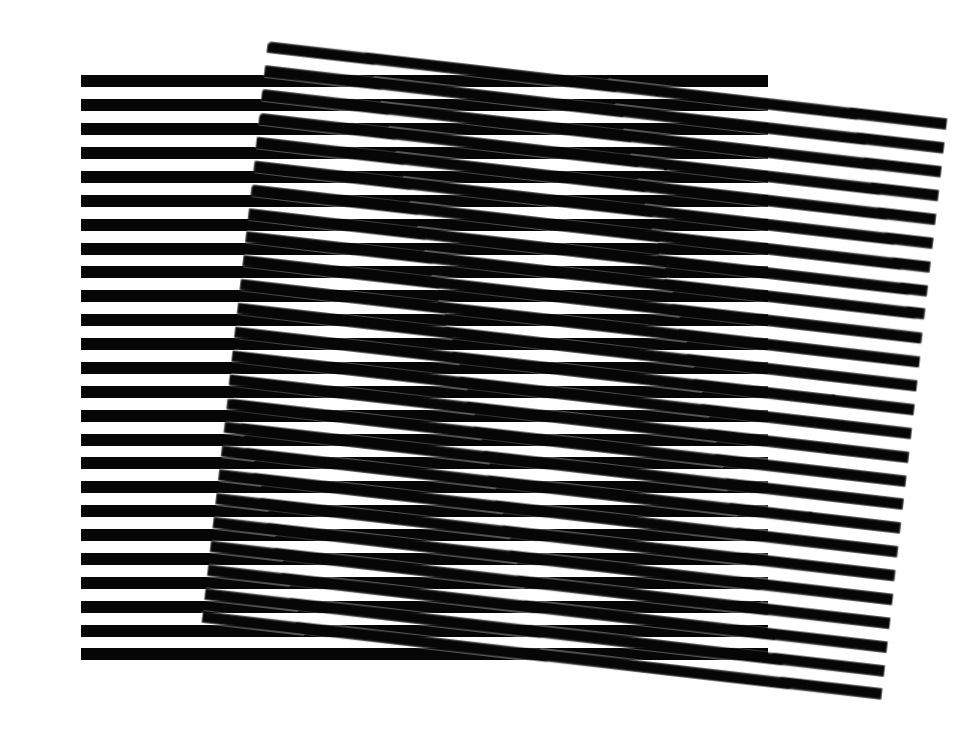
\includegraphics[scale=0.5]{figures/moire.png}
    \caption{Moir\'{e} Fringes}
    \label{fig:moire}
\end{figure}

In order to correctly interpret this interference effect, and reconstruct a super-resolved image,
multiple images need to be acquired from the microscope and analysed in the Fourier domain.
When reconstructed properly, there will be an improvement of lateral resolution in the direction of the k-vector of the pattern.
Therefore, when acquiring images for 2D SIM, 3 groups of images are almost always captured,
with the patterns angled $2\pi/3$ from eachother, to obtain an (almost) isotropic improvement in \textit{lateral} resolution,
and the same is true in 3D SIM.
Within these groups, the images are acquired with the illumination pattern having a different phase each time.

The reconstruction involes six key steps:
\begin{enumerate}
    \item Parameter estimation,
    \item Fourier transform,
    \item Band separation,
    \item Wiener filtering,
    \item Apodization, and,
    \item Inverse Fourier transform
\end{enumerate}

Parameter estimation is primarily concerned with the position of the illumination pattern,
including the phase, angle, and modulation depth.
This is more accurate than measuring these quantities in the physical system which would require high degree of care and precision.
Then the image is converted to the frequency domain.
Denoting the image intensity by $D(\vec{r})$, the pattern k-vector and phase by $\vec{p}$, $\phi_n$,
the modulation depth by $a_m$, the density of the fluorescent substance as $S(\vec{r})$ and the point-spread function by $H(\vec{r})$,
we see that the effect of the optical system on the `true' ground-truth structure $S$ is to multiply it with the excitation pattern,
and then convolve with the point-spread function:

\[D_n(\vec{r}) = \sum_{m=-M}^{M}{S(\vec{r})a_m\exp(im(2\pi\vec{p}\cdot\vec{r}+\phi_n))\otimes H(\vec{r})}\]

Utilising the Convolution Theorem this becomes

\[\tilde{D}_n(\vec{r}) = \sum_{m=-M}^{M}{\exp(im\phi_n)a_m\tilde{S}(\vec{k}-m\vec{p})\tilde{O}(\vec{k})}\]

In turn, with sufficient acquired images at different phases, namely M, this can be used to solve a fully determined set of linear equations for

\[\tilde{S}(\vec{k}-m\vec{p})\tilde{O}(\vec{k})\qquad m=-M,\dots,M-1,M\]

This constitutes the band separation step, and explains why 2D SIM uses 3 sets of 3 images, while 3D SIM uses 3 sets of 5 images;
the number of different phases used in imaging must correspond to the number of delta peaks that represent the illumination pattern in Fourier space.

The steps of Wiener filtering and Apodization are used to combine the separated bands of the image,
whilst also adequately dealing with noise and artefacts that can occur.

fairSIM and parameters.

\subsection{Data}

In the research Li. et al. acquired pairs of high and low SNR images which were used to train the networks.
In order to avoid to acquire these images more quickly, and to avoid the need for image registration to align the pairs of images acquired,
the increased noise resulting from lowering the illumination dose was simulated in-silico.

The 2D data was acquired in the lab using a two-beam SIM microscope.
Two sets of samples were collected for this purpose: firstly a set of images of host cells infected with viruses,
and later some cells whose microtubules had been dyed.
In both cases the samples were illuminated with visible light at 488nm and 561nm.

This was generated with the help of another student's code.
The code was modified to include only the most essential parts, and to generate a 3D volume of SIM acquisition stacks (15 each)

\subsection{RCAN}
Use elsewhere

Diagram

\subsection{Pipeline}
Describe building from scratch (pytorch vs tflow)

Diagram

Software

Using CSD3, hardware, parallel -> serial

\section{Results}

\subsection{2D Data}

Parameter estimation

Generalizability

Tables of results, metrics

Images

\subsection{3D Data}

Axial resolution

Tables of results, metrics

Images

\section{Discussion}
Results/conclusions
Further work
What I learned
How I could have improved

\bibliographystyle{IEEEtran}
\bibliography{Biblio}

\appendix

\section{Statement on the use of auto-generation tools}

\section {High-Performance Computing Resources}

This work was performed using resources provided by the Cambridge Service for Data Driven Discovery (CSD3) operated by the University of Cambridge Research Computing Service (www.csd3.cam.ac.uk),
provided by Dell EMC and Intel using Tier-2 funding from the Engineering and Physical Sciences Research Council (capital grant EP/T022159/1),
and DiRAC funding from the Science and Technology Facilities Council (www.dirac.ac.uk).

\end{document}
